\documentclass[12pt]{article}

\usepackage{hcmus-report-template}

% Disable indentation on new paragraphs
\setlength{\parindent}{0pt}

% Line spacing 1.5
\renewcommand{\baselinestretch}{1.5}

% Optional: graphic path
% \graphicspath{PATH_TO_GRAPHIC_FOLDER}

% To use Times font family, uncomment this row
% \usepackage{mathptmx}

% To use roman section / subsection, uncomment these rows
% \renewcommand{\thesection}{\Roman{section}}
% \renewcommand{\thesubsection}{\thesection.\Roman{subsection}}
% ===========================================

% Define course name, report name and report title.
\newcommand{\coursename}{Khai thác dữ liệu và ứng dụng}
\newcommand{\reportname}{Khai thác tập phổ biến}
\newcommand{\reporttitle}{Đồ án 2}

\newcommand{\studentname}{22120457 - Khưu Hải Châu\\23122006 - Lưu Thượng Hồng\\23122020 - Nguyễn Thiên Ấn\\23122034 - Lê Nguyên Khang\\23122036 - Nguyễn Ngọc Khoa}
\newcommand{\teachername}{GS.TS. Lê Hoài Bắc\\ThS. Lê Nhựt Nam}

% Header
\lhead{\reporttitle}
\rhead{
Trường Đại học Khoa học Tự nhiên - ĐHQG HCM\\
\coursename
}

% % Footer
% \newcommand{\leftfooter}{\LaTeX\ by \href{https://github.com/trhgquan}{Quan, Tran Hoang}}
% \lfoot{\leftfooter}
% test

% ============ DOCUMENT ============
\begin{document}

\pagenumbering{roman}
\input{content/title.tex}

\tableofcontents
\pagebreak
\listoftables
\pagebreak
\listoffigures
\pagebreak

\pagenumbering{arabic}
\setcounter{page}{1}

\section{Giới thiệu}
\label{sec:introduction}

Khai thác tập phổ biến (Frequent Itemset Mining, FIM) là một bài toán nền tảng trong khai thác dữ liệu giao dịch. Với một cơ sở dữ liệu gồm nhiều giao dịch, mục tiêu của FIM là tìm các nhóm item xuất hiện cùng nhau đủ thường xuyên theo một ngưỡng hỗ trợ tối thiểu. Kết quả của bài toán này thường được dùng làm đầu vào cho luật kết hợp, phân tích giỏ hàng, phát hiện mẫu trong log hệ thống, hoặc phân tích các tổ hợp đặc trưng trong dữ liệu sinh học.

Trong đồ án này, thuật toán nhóm lựa chọn là FP-Max, một thuật toán khai thác \textit{maximal frequent itemsets} (tập phổ biến tối đại) \cite{Grahne2003FPMax}. FP-Max không đứng riêng lẻ: thuật toán dựa trên FP-tree và các thao tác conditional pattern base của FP-Growth để nén dữ liệu, dựng cây điều kiện và tỉa nhánh. Vì vậy, nhóm phải cài đặt FP-tree/FP-Growth như phần nền tảng bắt buộc trước khi cài FP-Max. Nói cách khác, FP-Growth trong báo cáo này là prerequisite và engine trung gian; FP-Max mới là thuật toán chính của đề tài.

SPMF trong báo cáo không phải là một thuật toán nhóm chọn, mà là một thư viện Java mã nguồn mở về khai thác mẫu (Sequential Pattern Mining Framework) \cite{FournierViger2014SPMF}. Đề bài yêu cầu so sánh với SPMF vì thư viện này có các cài đặt tham chiếu phổ biến cho nhiều thuật toán FIM. Nhóm dùng SPMF như mốc đối chiếu output và thời gian chạy: nếu kết quả của phần FP-tree/FP-Growth nền khớp SPMF, ta có thêm cơ sở để tin rằng các support và cây điều kiện dùng trong FP-Max được xây đúng.

Báo cáo được tổ chức như sau. Mục \ref{sec:theory} trình bày các định nghĩa hình thức của FIM, FP-tree/FP-Growth như nền tảng của FP-Max, giả mã FP-Max và phân tích độ phức tạp. Mục \ref{sec:example} minh hoạ quá trình xây FP-tree rồi rút ra maximal itemsets. Mục \ref{sec:implementation} mô tả cài đặt Julia, trong đó FP-Growth là module nền và FP-Max là module khai thác chính. Mục \ref{sec:evaluation} trình bày kiểm thử, đối chiếu SPMF cho tầng frequent-itemset engine và đánh giá hiệu năng. Mục \ref{sec:application} áp dụng phần frequent-itemset engine vào phân tích giỏ hàng trên tập Groceries để sinh luật kết hợp.

\section{Phân công công việc}
\label{sec:job-distribution}

\begin{table}[H]
    \centering
    \caption{Bảng phân công công việc của nhóm}
    \begin{tabular}{l l p{7cm}}
        \toprule
        MSSV & Họ và tên & Công việc \\
        \midrule
        22120457 & Khưu Hải Châu    & Nghiên cứu lý thuyết FP-Growth, FP-Max và viết Chương 1 \\
        23122006 & Lưu Thượng Hồng  & Cài đặt FP-Growth cơ bản, parser, I/O và CLI Julia \\
        23122020 & Nguyễn Thiên Ấn  & Cài đặt FP-Growth tối ưu, unit test và đối chiếu SPMF \\
        23122034 & Lê Nguyên Khang  & Thiết kế thực nghiệm, đo thời gian/bộ nhớ và sinh biểu đồ \\
        23122036 & Nguyễn Ngọc Khoa & Ứng dụng Groceries, tổng hợp báo cáo và kiểm tra PDF \\
        \bottomrule
    \end{tabular}
\end{table}


\section{Nền tảng lý thuyết}

\subsection{Bài toán Frequent Itemset Mining}

\subsection{Thuật toán FPMax}
\section{Ví dụ minh họa}
\label{sec:example}

\subsection{Ví dụ 1: CSDL cơ sở}

Xét cơ sở dữ liệu $D$ gồm 5 giao dịch trong Bảng \ref{tab:toy-db}. Nhóm chọn minsup tương đối $\theta = 0.6$, do đó minsup tuyệt đối là $\lceil 0.6 \times 5 \rceil = 3$.

\begin{table}[H]
    \centering
    \caption{CSDL toy dùng để minh hoạ FP-Max.}
    \label{tab:toy-db}
    \begin{tabular}{c c}
        \toprule
        Giao dịch & Item \\
        \midrule
        $T_1$ & $\{1,3,4\}$ \\
        $T_2$ & $\{2,3,5\}$ \\
        $T_3$ & $\{1,2,3,5\}$ \\
        $T_4$ & $\{2,5\}$ \\
        $T_5$ & $\{1,2,3,5\}$ \\
        \bottomrule
    \end{tabular}
\end{table}

Bước đầu tiên là đếm support của từng item. Kết quả là $\operatorname{sup}(1)=3$, $\operatorname{sup}(2)=4$, $\operatorname{sup}(3)=4$, $\operatorname{sup}(4)=1$, $\operatorname{sup}(5)=4$. Vì minsup tuyệt đối bằng 3, item $4$ bị loại. Để dựng FP-tree, các item còn lại trong mỗi giao dịch được sắp theo support giảm dần, nếu bằng nhau thì theo mã item tăng dần: $2 \prec 3 \prec 5 \prec 1$.

\begin{table}[H]
    \centering
    \caption{Các giao dịch sau bước tỉa và sắp thứ tự để dựng FP-tree.}
    \label{tab:toy-ordered}
    \begin{tabular}{c c c}
        \toprule
        Giao dịch & Sau khi loại item không phổ biến & Sau khi sắp theo thứ tự FP-tree \\
        \midrule
        $T_1$ & $\{1,3\}$ & $[3,1]$ \\
        $T_2$ & $\{2,3,5\}$ & $[2,3,5]$ \\
        $T_3$ & $\{1,2,3,5\}$ & $[2,3,5,1]$ \\
        $T_4$ & $\{2,5\}$ & $[2,5]$ \\
        $T_5$ & $\{1,2,3,5\}$ & $[2,3,5,1]$ \\
        \bottomrule
    \end{tabular}
\end{table}

Chèn tuần tự các giao dịch trong Bảng \ref{tab:toy-ordered} tạo ra FP-tree trong Hình \ref{fig:fptree-toy-ex}.

\begin{figure}[H]
    \centering
    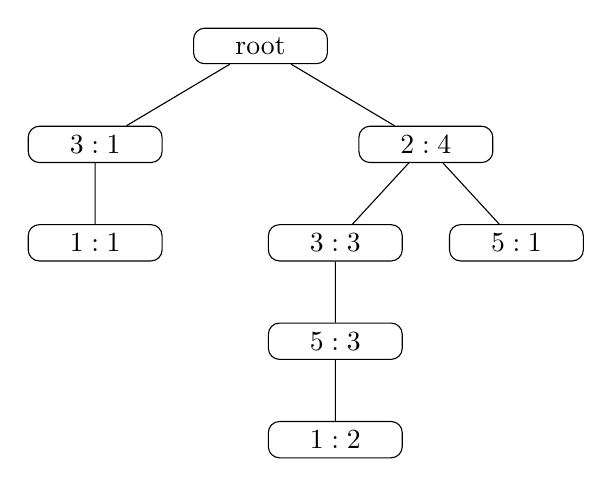
\begin{tikzpicture}[
        level distance=1.25cm,
        level 1/.style={sibling distance=4.2cm},
        level 2/.style={sibling distance=2.3cm},
        level 3/.style={sibling distance=1.8cm},
        every node/.style={draw, rounded corners, align=center, minimum width=1.7cm}
    ]
    \node {root}
        child { node {$3:1$}
            child { node {$1:1$} }
        }
        child { node {$2:4$}
            child { node {$3:3$}
                child { node {$5:3$}
                    child { node {$1:2$} }
                }
            }
            child { node {$5:1$} }
        };
    \end{tikzpicture}
    \caption{FP-tree cho CSDL toy Bảng \ref{tab:toy-db} sau bước tỉa và sắp thứ tự (Bảng \ref{tab:toy-ordered}).}
    \label{fig:fptree-toy-ex}
\end{figure}

Khác với FP-Growth, FP-Max duyệt header table theo thứ tự support \emph{tăng dần}, tức $1 \prec 2 \prec 3 \prec 5$ (item $1$ có support $3$, ba item còn lại có support $4$ nên xếp theo mã item). Bảng \ref{tab:toy-fpmax} ghi lại từng bước: head đang xét, conditional pattern base, tail (các item còn đủ support trong base), candidate tối đại sinh ra, và trạng thái danh sách MFI sau bước đó.

\begin{table}[H]
    \centering
    \caption{Vòng đệ quy FP-Max trên ví dụ cơ sở. Mỗi candidate được hợp nhất vào danh sách MFI theo quy tắc loại tập con nghiêm ngặt.}
    \label{tab:toy-fpmax}
    \small
    \begin{tabular}{c c c c c}
        \toprule
        Head & Conditional pattern base & Tail & Candidate & MFI sau bước \\
        \midrule
        $1$ & $(3):1,\ (2,3,5):2$ & $\{3\}$ & $\{1,3\}$ & $\{1,3\}$ \\
        $2$ & $\emptyset$ & $\emptyset$ & $\{2\}$ & $\{1,3\},\{2\}$ \\
        $3$ & $(2):3$ & $\{2\}$ & $\{2,3\}$ & $\{1,3\},\{2,3\}$ \\
        $5$ & $(2,3):3,\ (2):1$ & $\{2,3\}$ & $\{2,3,5\}$ & $\{1,3\},\{2,3,5\}$ \\
        \bottomrule
    \end{tabular}
\end{table}

Diễn giải các bước trong Bảng \ref{tab:toy-fpmax}. Khi xét head $\{1\}$, conditional pattern base gồm đường $(3)$ với count $1$ và đường $(2,3,5)$ với count $2$; chỉ item $3$ đạt support $3$ nên tail là $\{3\}$. Cây điều kiện co thành một đường, sinh candidate $\{1,3\}$ và khởi tạo MFI. Head $\{2\}$ có base rỗng (node $2$ nằm ngay dưới root) nên tạm thời cho candidate $\{2\}$. Đến head $\{3\}$, base $(2):3$ cho tail $\{2\}$ và candidate $\{2,3\}$; vì $\{2\}$ là tập con nghiêm ngặt của $\{2,3\}$ nên $\{2\}$ bị loại khỏi MFI. Cuối cùng head $\{5\}$ có base $(2,3):3$ và $(2):1$; tail $\{2,3\}$, cây điều kiện single-path cho candidate $\{2,3,5\}$, làm $\{2,3\}$ bị loại. Danh sách MFI hội tụ về hai phần tử.

Sau khi tính lại support trên $D$, tập kết quả của FP-Max là:
\[
    \{1,3\}:3, \qquad \{2,3,5\}:3.
\]

Để kiểm tra chéo thủ công, ta liệt kê toàn bộ tập phổ biến từ các item $\{1,2,3,5\}$: các đơn item $\{1\}:3,\{2\}:4,\{3\}:4,\{5\}:4$; các cặp $\{1,3\}:3,\{2,3\}:3,\{2,5\}:4,\{3,5\}:3$; và bộ ba $\{2,3,5\}:3$ (xuất hiện trong $T_2,T_3,T_5$). Trong chín tập phổ biến này, chỉ $\{1,3\}$ và $\{2,3,5\}$ là không có siêu tập phổ biến: mọi tập còn lại đều là tập con của một trong hai. Kết quả thủ công trùng khớp với đầu ra của FP-Max, và cũng đúng với cài đặt FPMax tham chiếu trong SPMF.

\subsection{Ví dụ 2: Tỉa theo siêu tập}

Trường hợp đặc biệt quan trọng của FP-Max là phép tỉa theo siêu tập: khi $head \cup tail$ đã nằm trong một MFI có sẵn, cả nhánh đệ quy bị cắt mà không cần dựng conditional FP-tree. Ví dụ này được thiết kế để phép tỉa thực sự kích hoạt.

Xét CSDL trong Bảng \ref{tab:prune-db} với $\theta = 0.5$, minsup tuyệt đối bằng 3.

\begin{table}[H]
    \centering
    \caption{CSDL thiết kế để kích hoạt phép tỉa theo siêu tập trong FP-Max.}
    \label{tab:prune-db}
    \begin{tabular}{c c}
        \toprule
        Giao dịch & Item \\
        \midrule
        $T_1$ & $\{a,b,c\}$ \\
        $T_2$ & $\{a,b,c\}$ \\
        $T_3$ & $\{a,b,c\}$ \\
        $T_4$ & $\{a,b,d\}$ \\
        $T_5$ & $\{a,b,d\}$ \\
        $T_6$ & $\{a,b,d\}$ \\
        \bottomrule
    \end{tabular}
\end{table}

Support của các item là $\operatorname{sup}(a)=6$, $\operatorname{sup}(b)=6$, $\operatorname{sup}(c)=3$, $\operatorname{sup}(d)=3$; tất cả đều đạt ngưỡng. Thứ tự dựng cây theo support giảm dần là $a,b,c,d$, cho FP-tree trong Hình \ref{fig:fptree-prune}.

\begin{figure}[H]
    \centering
    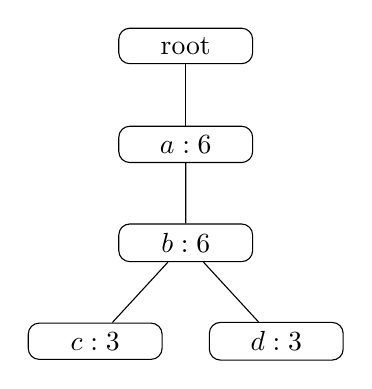
\begin{tikzpicture}[
        level distance=1.25cm,
        level 1/.style={sibling distance=3cm},
        level 2/.style={sibling distance=3cm},
        level 3/.style={sibling distance=2.3cm},
        every node/.style={draw, rounded corners, align=center, minimum width=1.7cm}
    ]
    \node {root}
        child { node {$a:6$}
            child { node {$b:6$}
                child { node {$c:3$} }
                child { node {$d:3$} }
            }
        };
    \end{tikzpicture}
    \caption{FP-tree cho CSDL Bảng \ref{tab:prune-db}. Node $b$ phân nhánh thành $c$ và $d$ nên cây không phải single-path.}
    \label{fig:fptree-prune}
\end{figure}

Vì node $b$ có hai con, cây không phải single-path nên thuật toán đi vào vòng đệ quy theo từng item. Header được duyệt theo support tăng dần: $c,d,a,b$ (hai item hiếm $c,d$ trước, hai item phổ biến $a,b$ sau). Bảng \ref{tab:prune-trace} ghi lại diễn biến.

\begin{table}[H]
    \centering
    \caption{Vòng đệ quy FP-Max trên CSDL Bảng \ref{tab:prune-db}. Hai item cuối bị tỉa nhờ kiểm tra siêu tập.}
    \label{tab:prune-trace}
    \small
    \begin{tabular}{c c c c l}
        \toprule
        Head & Conditional pattern base & $head\cup tail$ & Hành động & MFI sau bước \\
        \midrule
        $c$ & $(a,b):3$ & $\{a,b,c\}$ & dựng cây, candidate $\{a,b,c\}$ & $\{a,b,c\}$ \\
        $d$ & $(a,b):3$ & $\{a,b,d\}$ & dựng cây, candidate $\{a,b,d\}$ & $\{a,b,c\},\{a,b,d\}$ \\
        $a$ & $\emptyset$ & $\{a\}$ & $\{a\}\subseteq\{a,b,c\}$ $\Rightarrow$ tỉa & $\{a,b,c\},\{a,b,d\}$ \\
        $b$ & $(a):6$ & $\{a,b\}$ & $\{a,b\}\subseteq\{a,b,c\}$ $\Rightarrow$ tỉa & $\{a,b,c\},\{a,b,d\}$ \\
        \bottomrule
    \end{tabular}
\end{table}

Hai item hiếm $c$ và $d$ được xử lý trước, mỗi item có conditional pattern base $(a,b):3$ nên sinh hai tối đại $\{a,b,c\}$ và $\{a,b,d\}$. Khi đến item $b$, conditional pattern base là $(a):6$ cho tail $\{a\}$; vì $head \cup tail = \{a,b\}$ đã là tập con của MFI $\{a,b,c\}$, thuật toán cắt cả nhánh và \emph{không} dựng conditional FP-tree cho $b$ --- đây chính là chỗ tỉa tiết kiệm công sức. Item $a$ tương tự bị tỉa với $head\cup tail=\{a\}$. Tập kết quả là $\{a,b,c\}:3$ và $\{a,b,d\}:3$.

Trường hợp này làm rõ điểm khác biệt cốt lõi giữa FP-Max và FP-Growth. FP-Growth buộc phải xuất ra mọi tập phổ biến --- ở đây gồm $\{a\},\{b\},\{a,b\},\{a,c\},\{b,c\},\{a,b,c\},\dots$ với tổng cộng mười tập --- trong khi FP-Max chỉ giữ hai tối đại và bỏ qua phần lớn không gian nhờ phép tỉa. Cực điểm của hiệu ứng này là khi FP-tree co thành một đường đi dài $k$: FP-Growth sinh $2^k-1$ tập phổ biến, còn FP-Max nhận diện single-path và trả về đúng một tối đại; Ví dụ 3 minh hoạ cụ thể trường hợp đó. Đây là lý do FP-Max đặc biệt hiệu quả trên dữ liệu dày, nơi số tập phổ biến lớn theo cấp số mũ nhưng số tập tối đại nhỏ hơn nhiều.

\subsection{Ví dụ 3: FP-tree single-path}
\label{sec:example-singlepath}

Trường hợp đặc biệt thứ hai, và cũng là nguồn gốc của phần lớn hiệu năng FP-Max, là khi \emph{toàn bộ} FP-tree (hoặc một conditional FP-tree) co lại thành một đường đi duy nhất. Khi đó mọi item trên đường đều cùng xuất hiện trong các giao dịch sinh ra đường đó, nên hợp của chúng đã là một tập phổ biến; FP-Max nhận diện cấu trúc single-path và trả thẳng \emph{một} tối đại duy nhất mà không cần đệ quy qua từng head. Ví dụ này được thiết kế để chính cây gốc là single-path.

Xét CSDL trong Bảng \ref{tab:single-db} với $\theta = 0.5$, minsup tuyệt đối bằng 2.

\begin{table}[H]
    \centering
    \caption{CSDL thiết kế để FP-tree gốc co thành một đường đi duy nhất.}
    \label{tab:single-db}
    \begin{tabular}{c c}
        \toprule
        Giao dịch & Item \\
        \midrule
        $T_1$ & $\{a,b,c\}$ \\
        $T_2$ & $\{a,b,c\}$ \\
        $T_3$ & $\{a,b\}$ \\
        $T_4$ & $\{a\}$ \\
        \bottomrule
    \end{tabular}
\end{table}

Support của các item là $\operatorname{sup}(a)=4$, $\operatorname{sup}(b)=3$, $\operatorname{sup}(c)=2$; cả ba đều đạt ngưỡng. Mỗi giao dịch là tập con của giao dịch dài hơn (cấu trúc lồng nhau $\{a\}\subset\{a,b\}\subset\{a,b,c\}$), nên khi chèn theo thứ tự support giảm dần $a,b,c$, mọi giao dịch dùng chung tiền tố và FP-tree co thành một đường đi duy nhất trong Hình \ref{fig:fptree-single}.

\begin{figure}[H]
    \centering
    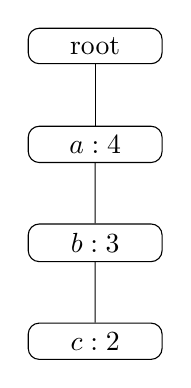
\begin{tikzpicture}[
        level distance=1.25cm,
        level 1/.style={sibling distance=3cm},
        every node/.style={draw, rounded corners, align=center, minimum width=1.7cm}
    ]
    \node {root}
        child { node {$a:4$}
            child { node {$b:3$}
                child { node {$c:2$} }
            }
        };
    \end{tikzpicture}
    \caption{FP-tree cho CSDL Bảng \ref{tab:single-db}. Không node nào phân nhánh nên cây là single-path, FP-Max trả thẳng một tối đại.}
    \label{fig:fptree-single}
\end{figure}

Vì root chỉ có một con và không node nào phân nhánh, thuật toán phát hiện single-path ngay tại lời gọi gốc. Thay vì duyệt header table và đệ quy theo từng head, FP-Max gom mọi item trên đường đạt minsup thành một candidate duy nhất $\{a,b,c\}$ với support bằng count nhỏ nhất trên đường ($\operatorname{sup}(c)=2$), rồi hợp vào danh sách MFI. Tập kết quả là:
\[
    \{a,b,c\}:2.
\]

Đối chiếu chi phí giữa hai thuật toán làm rõ giá trị của lối tắt single-path. Trên cùng CSDL này, FP-Growth phải liệt kê toàn bộ $2^3-1=7$ tập phổ biến trong Bảng \ref{tab:single-compare}; FP-Max chỉ giữ lại đúng tập tối đại bao trùm cả bảy. Khi đường dài $k$ thay vì $3$, khoảng cách này nới rộng thành $2^k-1$ so với $1$ --- đúng hành vi cấp số mũ đã nêu ở cuối Ví dụ 2.

\begin{table}[H]
    \centering
    \caption{So sánh đầu ra trên CSDL single-path Bảng \ref{tab:single-db}: FP-Growth liệt kê mọi tập con, FP-Max chỉ giữ tối đại.}
    \label{tab:single-compare}
    \begin{tabular}{l l}
        \toprule
        Thuật toán & Đầu ra \\
        \midrule
        FP-Growth & $\{a\}:4,\ \{b\}:3,\ \{c\}:2,\ \{a,b\}:3,\ \{a,c\}:2,\ \{b,c\}:2,\ \{a,b,c\}:2$ \\
        FP-Max & $\{a,b,c\}:2$ \\
        \bottomrule
    \end{tabular}
\end{table}

\section{Cài đặt}

\subsection{Môi trường và tổ chức mã nguồn}

Cài đặt chính của nhóm sử dụng Julia theo đúng ưu tiên của đề bài. Mã nguồn được tổ chức như một package tên \texttt{FrequentItemsetMining}, trong đó file \texttt{src/FrequentItemsetMining.jl} là module entry và include các file con. Bố cục chính của repo như sau:

\begin{itemize}
    \item \texttt{src/structures.jl}: định nghĩa \texttt{Transaction}, \texttt{DataLoader}, \texttt{FPNode}, \texttt{FPNodeOpt}.
    \item \texttt{src/data\_loader.jl}: đọc dữ liệu giao dịch, hỗ trợ dòng item cách nhau bằng khoảng trắng theo định dạng SPMF và dòng có dấu phẩy.
    \item \texttt{src/algorithm/fp\_growth.jl}: cài đặt FP-Growth cơ bản.
    \item \texttt{src/algorithm/fp\_growth\_opt.jl}: cài đặt FP-Growth tối ưu.
    \item \texttt{src/algorithm/fp\_max.jl}: cài đặt FP-Max.
    \item \texttt{src/io.jl}: xuất itemsets theo dạng \texttt{item item ... \#SUP: count}.
    \item \texttt{main.jl}: giao diện dòng lệnh.
    \item \texttt{test/}: bộ unit test correctness và benchmark smoke test.
    \item \texttt{experiments/}: script đối chiếu SPMF, sinh CSV và sinh hình cho Chương 4.
\end{itemize}

Lệnh chạy chương trình có dạng:

\begin{lstlisting}[language=bash, caption={Cách chạy chương trình từ dòng lệnh.}]
julia --project=. main.jl <input_path> <minsup> [fp-growth|fp-growth-opt|fp-max] [output_path]
\end{lstlisting}

Ví dụ, để khai thác tập phổ biến trên CSDL đồ chơi với ngưỡng $0.6$:

\begin{lstlisting}[language=bash, caption={Ví dụ chạy FP-Growth tối ưu.}]
julia --project=. main.jl data/toy/test_1.txt 0.6 fp-growth-opt output.txt
\end{lstlisting}

\subsection{Cài đặt FP-Growth cơ bản}

Bản cơ bản dùng node lưu item dạng \texttt{String}. Mỗi node có \texttt{count}, con trỏ \texttt{parent} và tập \texttt{children}. Khi chèn item vào một node cha, chương trình duyệt các con hiện có để tìm child cùng item; nếu có thì tăng count, nếu không thì tạo node mới. Sau khi xây cây, hàm \texttt{rebuild\_nodes\_table!} duyệt cây để dựng header table.

Quy trình \texttt{fit!} của \texttt{FPGrowth} gồm bốn bước. Thứ nhất, gom toàn bộ giao dịch và tính minsup tuyệt đối bằng $\lceil \theta n \rceil$. Thứ hai, đếm support từng item và loại item không đủ ngưỡng. Thứ ba, trong mỗi giao dịch, giữ lại item phổ biến và sắp theo \texttt{(-support, item)} để kết quả có thứ tự ổn định. Cuối cùng, chèn các giao dịch vào FP-tree.

Hàm \texttt{get\_frequent\_itemsets} khai thác từng item bằng \texttt{mine\_roads}. Với mỗi node của item đang xét, hàm đi ngược theo con trỏ cha để lấy đường tiền tố. Các đường tiền tố tạo thành conditional pattern base. Bản cơ bản sau đó đếm các item hợp lệ trong base, sinh các tổ hợp con của chúng và tính support bằng cách kiểm tra đường nào chứa tổ hợp đó. Cách này dễ kiểm chứng và phù hợp làm baseline, nhưng có thể tốn kém khi conditional base rộng vì phải enumerate nhiều tổ hợp.

\subsection{Cài đặt FP-Growth tối ưu}

Bản \texttt{FPGrowthOpt} giữ cùng API với bản cơ bản nhưng thay đổi cấu trúc dữ liệu và cách khai thác. Các item được mã hoá từ \texttt{String} sang \texttt{Int}. Mỗi node tối ưu lưu \texttt{item::Int}, \texttt{count::Int}, \texttt{parent}, và \texttt{children::Dict\{Int, FPNodeOpt\}}. Nhờ vậy thao tác tìm child khi chèn path có chi phí trung bình $O(1)$ thay vì duyệt tuyến tính qua tập con.

Các kỹ thuật tối ưu chính gồm:

\begin{itemize}
    \item \textbf{Integer encoding}: khai thác trên mã số nguyên và chỉ giải mã về chuỗi ở bước cuối.
    \item \textbf{Header table typed}: header ánh xạ \texttt{Int} sang danh sách node, giảm overhead so với item chuỗi.
    \item \textbf{Recursive conditional FP-tree}: khai thác đúng hướng FP-Growth chuẩn, tránh enumerate tổ hợp trên conditional base rộng như bản cơ bản.
    \item \textbf{Single-path shortcut}: nếu cây điều kiện chỉ có một nhánh, sinh trực tiếp mọi tổ hợp con của nhánh đó.
    \item \textbf{Tỉa sớm}: trong mỗi conditional pattern base, item có support nhỏ hơn minsup tuyệt đối bị loại trước khi dựng cây điều kiện.
    \item \textbf{Type-stable hot loop}: các trường dữ liệu được khai báo kiểu cụ thể và một số vòng lặp dùng \texttt{@inbounds} khi truy cập vector.
\end{itemize}

Output của bản tối ưu vẫn là \texttt{Dict\{Tuple\{Vararg\{String\}\}, Int\}}, giống bản cơ bản. Điều này giúp unit test có thể so sánh trực tiếp:

\begin{center}
\texttt{get\_frequent\_itemsets(FPGrowthOpt) == get\_frequent\_itemsets(FPGrowth)}
\end{center}

\subsection{Cài đặt FP-Max}

\texttt{FPMax} sử dụng \texttt{FPGrowth} để dựng cây ban đầu, đồng thời lưu lại toàn bộ giao dịch dưới dạng \texttt{Set\{String\}} để tính support của maximal itemsets ở bước cuối. Hàm \texttt{get\_maximal\_itemsets} duy trì danh sách các MFI dưới dạng vector các set. Khi có candidate mới, hàm \texttt{insert\_mfi!} bỏ qua candidate nếu nó là tập con của một MFI có sẵn; ngược lại, hàm xoá các MFI cũ là tập con nghiêm ngặt của candidate rồi thêm candidate mới.

Trong đệ quy FP-Max, nếu cây là single-path thì thuật toán hợp head hiện tại với toàn bộ item trên đường đi và cập nhật MFI. Nếu cây có nhiều nhánh, thuật toán xét các item trong header theo support tăng dần, tạo conditional pattern base, tìm tail còn phổ biến, rồi dùng kiểm tra $head \cup tail$ để tỉa các nhánh chắc chắn không sinh MFI mới.

\subsection{Kiểm thử tự động}

Bộ kiểm thử trong \texttt{test/test\_correctness.jl} gồm ba nhóm chính. Nhóm đầu kiểm tra parser với ba định dạng: \texttt{1, 2, 3}, \texttt{\{1, 2, 3\}}, và \texttt{1 2 3}. Nhóm thứ hai kiểm tra FP-Growth cơ bản trên CSDL đồ chơi ở Chương 2, kỳ vọng đúng 9 frequent itemsets với support tương ứng. Nhóm thứ ba kiểm tra FP-Max trên cùng CSDL, kỳ vọng hai maximal itemsets $\{1,3\}$ và $\{2,3,5\}$.

Ngoài ra, test đối chiếu \texttt{FPGrowthOpt} với \texttt{FPGrowth} trên \texttt{data/toy/test\_1.txt}, \texttt{data/toy/test\_2.txt} và \texttt{data/benchmark/chess.txt} ở nhiều giá trị minsup. Test benchmark trong \texttt{test/test\_benchmark.jl} đo thời gian và số byte cấp phát trên \texttt{chess} với minsup $0.9$, sau đó kiểm tra lại kết quả của bản tối ưu và bản cơ bản phải trùng nhau. Lệnh kiểm thử chuẩn là:

\begin{lstlisting}[language=bash, caption={Lệnh chạy bộ test.}]
julia --project=. test/runtests.jl
\end{lstlisting}

\subsection{Xử lý đầu vào và đầu ra}

Input chuẩn của đồ án là mỗi giao dịch trên một dòng, item cách nhau bằng khoảng trắng theo định dạng SPMF. Parser cũng hỗ trợ dòng có dấu phẩy để thuận tiện cho dữ liệu giỏ hàng. Output của \texttt{write\_itemsets} sắp các itemset theo độ dài và thứ tự từ điển, sau đó ghi mỗi dòng theo dạng:

\begin{lstlisting}[caption={Định dạng output itemset.}]
item1 item2 ... #SUP: support_count
\end{lstlisting}

Định dạng này tương thích với output của SPMF, giúp script thực nghiệm đọc kết quả của hai phía và so sánh từng itemset theo support.

\section{Thực nghiệm và đánh giá}
\label{sec:evaluation}

\subsection{Thiết lập thực nghiệm}

Thực nghiệm được thiết kế để kiểm tra sáu khía cạnh: tính đúng đắn so với SPMF FPMax, thời gian chạy theo minsup, số lượng tập tối đại theo minsup, bộ nhớ cấp phát, khả năng mở rộng theo số giao dịch, và ảnh hưởng của độ dài giao dịch trung bình. Kết quả được lưu trong các file CSV ở \texttt{experiments/results/}; hình minh hoạ được sinh vào \texttt{experiments/figures/}.

Các cài đặt được so sánh gồm:

\begin{itemize}
    \item \texttt{base}: baseline naive-maximal của nhóm --- khai thác toàn bộ tập phổ biến bằng \texttt{FPGrowthOpt} rồi lọc các tập tối đại.
    \item \texttt{opt}: FP-Max trực tiếp của nhóm --- khai thác tối đại có danh sách MFI và phép tỉa theo siêu tập.
    \item \texttt{spmf}: cài đặt FPMax trong thư viện SPMF \cite{FournierViger2014SPMF}, dùng làm tham chiếu.
\end{itemize}

Baseline naive-maximal phải vật chất hoá toàn bộ tập phổ biến trước khi lọc, nên không chạy ở các cấu hình có nguy cơ bùng nổ bộ nhớ, đặc biệt trên dữ liệu dày hoặc minsup thấp. Các cấu hình này được đánh dấu \texttt{skip} trong CSV thay vì ép chạy đến khi tiến trình bị lỗi; riêng \texttt{accidents} luôn skip base. Đây cũng chính là điểm khác biệt then chốt: FP-Max trực tiếp vẫn hoàn tất trong những vùng mà baseline không khả thi. Với Julia, thời gian được đo sau một lần warm-up để giảm ảnh hưởng của JIT; lượng cấp phát dùng cột \texttt{alloc\_bytes} từ \texttt{@timed}, còn peak memory thật được đo riêng bằng \texttt{Sys.maxrss} trong tiến trình độc lập (xem Mục Bộ nhớ). Với SPMF, thời gian và bộ nhớ lấy từ log của chương trình Java.

\subsection{Tập dữ liệu benchmark}

Bảng \ref{tab:benchmark-datasets} tóm tắt các tập dữ liệu dùng trong thực nghiệm. Các tập dữ liệu này là benchmark phổ biến trong cộng đồng FIM, lấy từ kho dữ liệu FIMI \cite{Goethals2003FIMI}. Các số liệu trong bảng được tính trực tiếp từ file trong thư mục \texttt{data/benchmark}.

\begin{table}[H]
    \centering
    \caption{Các tập dữ liệu benchmark dùng trong Mục \ref{sec:evaluation}.}
    \label{tab:benchmark-datasets}
    \begin{tabular}{l r r r l}
        \toprule
        Dataset & \#Trans. & \#Items & AvgLen & Đặc điểm \\
        \midrule
        Chess & 3,196 & 75 & 37.00 & Dày, giao dịch dài \\
        Mushrooms & 8,416 & 119 & 23.00 & Dày, nhiều item đồng xuất hiện \\
        Retail & 88,162 & 16,470 & 10.31 & Thưa, dữ liệu bán lẻ thực \\
        T10I4D100K & 100,000 & 870 & 10.10 & Tổng hợp, thưa \\
        Accidents & 340,183 & 468 & 33.80 & Rất lớn và dày \\
        \bottomrule
    \end{tabular}
\end{table}

\subsection{Tính đúng đắn}

Kết quả trong \texttt{correctness.csv} cho thấy mọi cấu hình được kiểm tra đều khớp hoàn toàn với SPMF FPMax: \texttt{match\_ratio = 1.0} và \texttt{support\_mismatch = 0}, cho cả bản \texttt{base} lẫn \texttt{opt}. Bảng \ref{tab:correctness-summary} liệt kê một số điểm đại diện, trong đó \#Ours và \#SPMF là số tập tối đại.

\begin{table}[H]
    \centering
    \caption{Kết quả correctness đại diện khi so số tập tối đại với SPMF FPMax.}
    \label{tab:correctness-summary}
    \begin{tabular}{l r l r r r}
        \toprule
        Dataset & minsup & Algo & \#Ours & \#SPMF & Match ratio \\
        \midrule
        Chess & 0.80 & base/opt & 226 & 226 & 1.0 \\
        Mushrooms & 0.25 & base/opt & 110 & 110 & 1.0 \\
        Retail & 0.01 & base/opt & 78 & 78 & 1.0 \\
        T10I4D100K & 0.01 & base/opt & 370 & 370 & 1.0 \\
        Accidents & 0.70 & opt & 23 & 23 & 1.0 \\
        \bottomrule
    \end{tabular}
\end{table}

Kết quả này xác nhận ba điểm. Thứ nhất, parser, cách tính minsup tuyệt đối và support của nhóm tương thích với SPMF trên dữ liệu benchmark. Thứ hai, cài đặt FP-Max trực tiếp cho đúng tập tối đại như cài đặt tham chiếu. Thứ ba, hai chiến lược \texttt{base} và \texttt{opt} của nhóm cho cùng kết quả, nên phép tỉa theo siêu tập không làm mất tối đại nào.

\subsection{Thời gian chạy theo minsup}

Hình \ref{fig:time-chess} đến Hình \ref{fig:time-t10} cho thấy thời gian chạy khi minsup giảm. Xu hướng chung là minsup càng thấp thì số tập tối đại càng tăng và thời gian chạy tăng theo. Điều này phù hợp với phân tích lý thuyết: khi ngưỡng thấp, nhiều item sống sót qua bước tỉa hơn, conditional tree rộng hơn và số tối đại lớn hơn.

\begin{figure}[H]
    \centering
    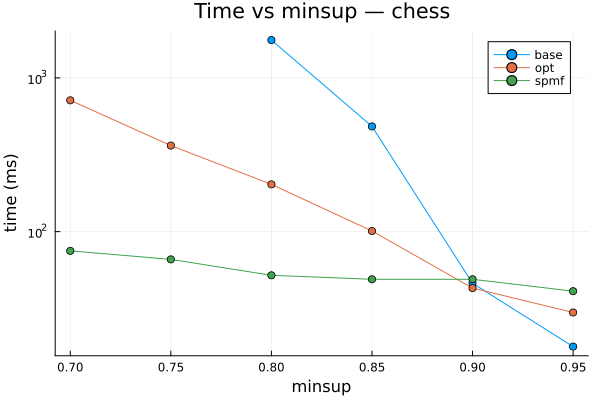
\includegraphics[width=0.85\linewidth]{../experiments/figures/time_chess.png}
    \caption{Thời gian chạy theo minsup trên Chess.}
    \label{fig:time-chess}
\end{figure}

Trên Chess, FP-Max trực tiếp (\texttt{opt}) thể hiện lợi thế rõ ở vùng output lớn. Tại minsup $0.80$, baseline naive-maximal mất 1762.92 ms trong khi \texttt{opt} chỉ mất 203.07 ms, nhanh hơn khoảng 8.68 lần; ở các ngưỡng thấp hơn ($0.75$, $0.70$) baseline bị skip vì mine-all bùng nổ, còn \texttt{opt} vẫn chạy (714.94 ms ở minsup $0.70$ với 891 tối đại). Khi minsup rất cao như $0.95$, output chỉ còn 11 tối đại nên chi phí cố định chiếm ưu thế và baseline lại nhanh hơn đôi chút (17.88 ms so với 29.81 ms). So với SPMF, \texttt{opt} vẫn chậm hơn (203.07 ms so với 52 ms ở minsup $0.80$), phản ánh khoảng cách giữa cài đặt học thuật và thư viện Java đã tối ưu lâu dài.

\begin{figure}[H]
    \centering
    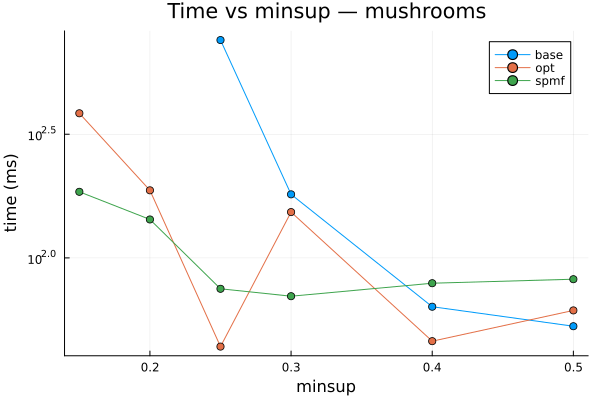
\includegraphics[width=0.85\linewidth]{../experiments/figures/time_mushrooms.png}
    \caption{Thời gian chạy theo minsup trên Mushrooms.}
    \label{fig:time-mushrooms}
\end{figure}

Hình \ref{fig:time-mushrooms} thể hiện xu hướng tương tự trên Mushrooms. Tại minsup $0.25$, \texttt{opt} nhanh hơn baseline khoảng 4.84 lần (147.81 ms so với 715.35 ms); ở minsup $0.30$ tỉ lệ thu hẹp còn 1.66 lần. Ở các ngưỡng cao ($0.4$, $0.5$) khi output nhỏ, hai bản xấp xỉ nhau và chi phí dựng cây cùng JIT chi phối.

\begin{figure}[H]
    \centering
    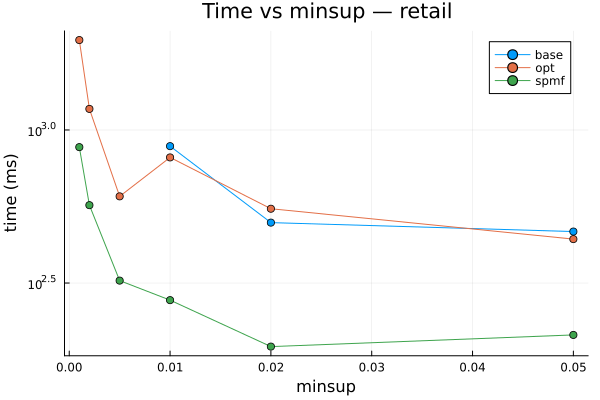
\includegraphics[width=0.85\linewidth]{../experiments/figures/time_retail.png}
    \caption{Thời gian chạy theo minsup trên Retail.}
    \label{fig:time-retail}
\end{figure}

Hình \ref{fig:time-retail} cho thấy một bức tranh ngược lại trên dữ liệu thưa. Vì Retail thưa, số tập phổ biến không lớn hơn số tối đại bao nhiêu nên phép tỉa của FP-Max ít có tác dụng, trong khi chi phí cài đặt --- node dạng \texttt{String} và bước tính lại support cho từng MFI trên toàn cơ sở dữ liệu --- lại lấn át. Tại minsup $0.01$, \texttt{opt} chậm hơn baseline (902.09 ms so với 548.92 ms). Ở minsup $0.001$, \texttt{opt} mất 18959.89 ms còn SPMF chỉ 1057 ms. Đây là điểm yếu rõ nhất của cài đặt FP-Max hiện tại và là động lực cho hướng tối ưu ở cuối mục.

\begin{figure}[H]
    \centering
    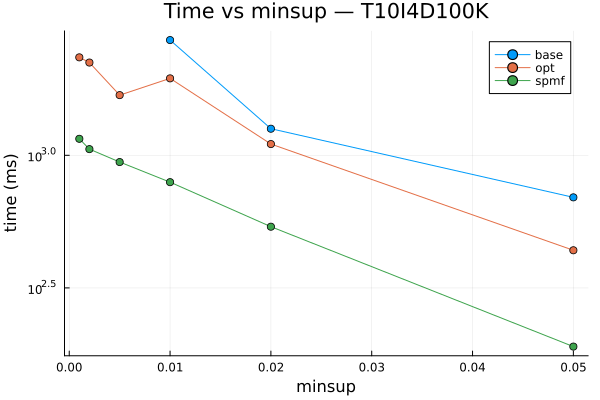
\includegraphics[width=0.85\linewidth]{../experiments/figures/time_T10I4D100K.png}
    \caption{Thời gian chạy theo minsup trên T10I4D100K.}
    \label{fig:time-t10}
\end{figure}

Trên T10I4D100K, vốn thưa và tổng hợp, xu hướng giống Retail: baseline nhanh hơn \texttt{opt} ở các điểm cả hai còn chạy (ví dụ minsup $0.01$: 1192.31 ms so với 4347.90 ms). Lợi ích nén tiền tố và tỉa siêu tập không đủ bù chi phí cài đặt trên dữ liệu thưa.

\begin{figure}[H]
    \centering
    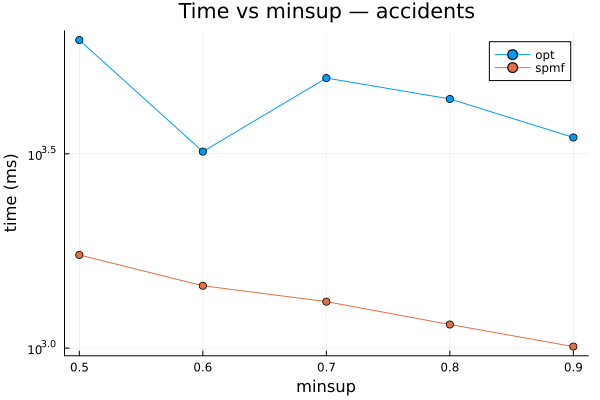
\includegraphics[width=0.85\linewidth]{../experiments/figures/time_accidents.png}
    \caption{Thời gian chạy theo minsup trên Accidents.}
    \label{fig:time-accidents}
\end{figure}

Hình \ref{fig:time-accidents} trình bày kết quả trên Accidents. Baseline bị bỏ qua hoàn toàn vì dữ liệu vừa lớn vừa dày khiến mine-all không khả thi --- đúng vùng mà FP-Max trực tiếp phát huy giá trị. \texttt{opt} chạy được ở mọi ngưỡng từ $0.9$ đến $0.5$, với thời gian từ 5.13 giây (minsup $0.9$, 1 tối đại) đến 20.23 giây (minsup $0.5$, 216 tối đại), chậm hơn SPMF khoảng 4--11 lần. Điểm yếu chính vẫn là cài đặt cấp phát nhiều object \texttt{String} cho conditional trees và tính lại support cho từng MFI.

\subsection{Số lượng tập tối đại theo minsup}

Hình \ref{fig:count-chess} và Hình \ref{fig:count-retail} minh hoạ quan hệ giữa minsup và số tập tối đại đầu ra. Chess tăng từ 11 tối đại ở minsup $0.95$ lên 891 tối đại ở minsup $0.70$. Retail tăng từ 4 tối đại ở minsup $0.05$ lên 3,452 tối đại ở minsup $0.001$.

\begin{figure}[H]
    \centering
    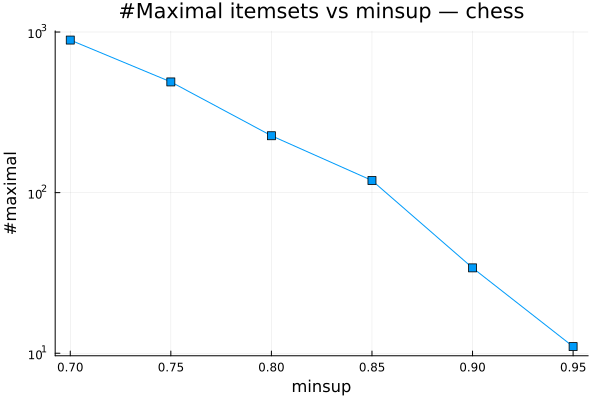
\includegraphics[width=0.82\linewidth]{../experiments/figures/count_chess.png}
    \caption{Số tập tối đại theo minsup trên Chess.}
    \label{fig:count-chess}
\end{figure}

\begin{figure}[H]
    \centering
    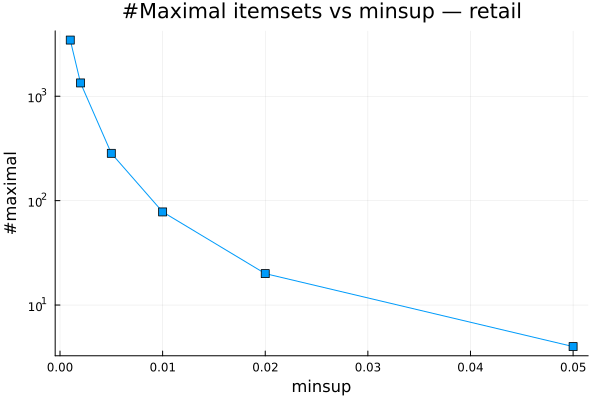
\includegraphics[width=0.82\linewidth]{../experiments/figures/count_retail.png}
    \caption{Số tập tối đại theo minsup trên Retail.}
    \label{fig:count-retail}
\end{figure}

Sự khác biệt giữa hai hình cho thấy độ dày dữ liệu ảnh hưởng mạnh đến output size. Chess có giao dịch dài và nhiều item đồng xuất hiện nên khi minsup giảm trong một khoảng hẹp, số tối đại tăng nhanh. Retail có nhiều item phân biệt nhưng giao dịch ngắn, vì vậy số tối đại chỉ tăng mạnh ở vùng minsup rất thấp. Đáng chú ý là số tập tối đại nhỏ hơn nhiều số tập phổ biến tương ứng: đây chính là lợi ích biểu diễn cô đọng mà FP-Max khai thác, và là lý do cài đặt trực tiếp khả thi trên Accidents trong khi baseline thì không.

\subsection{Bộ nhớ}

Hình \ref{fig:memory} so sánh lượng byte cấp phát giữa baseline và FP-Max tại một minsup trung bình của từng dataset. Trên dữ liệu dày, FP-Max cấp phát ít hơn hẳn: Chess ở minsup $0.85$ giảm từ 119.71 MB (base) xuống 25.23 MB (opt), khoảng 4.75 lần; Mushrooms ở minsup $0.30$ giảm từ 123.79 MB xuống 45.67 MB, khoảng 2.71 lần. Ngược lại, trên dữ liệu thưa FP-Max cấp phát nhiều hơn baseline: Retail ở minsup $0.02$ là 188.38 MB so với 116.27 MB, và T10I4D100K ở minsup $0.02$ là 434.60 MB so với 284.74 MB. Điều này nhất quán với phân tích thời gian: phép tỉa chỉ tiết kiệm khi có nhiều tập phổ biến không tối đại để cắt.

\begin{figure}[H]
    \centering
    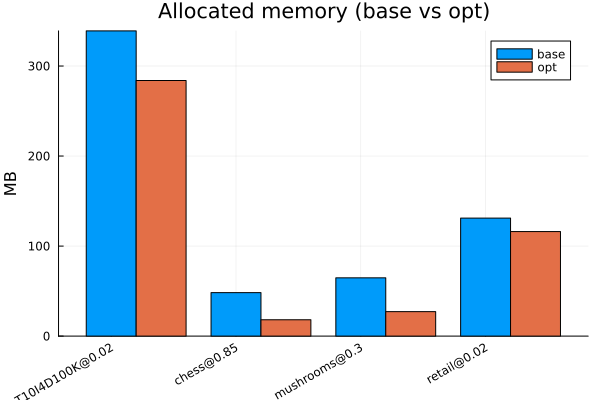
\includegraphics[width=0.85\linewidth]{../experiments/figures/memory.png}
    \caption{Bộ nhớ cấp phát của baseline naive-maximal và FP-Max tại minsup trung bình.}
    \label{fig:memory}
\end{figure}

Cột \texttt{alloc\_bytes} phản ánh tổng lượng cấp phát trong Julia, tức áp lực lên bộ thu gom rác (GC), chứ không phải dung lượng thường trú lớn nhất của tiến trình. Để đo trực tiếp peak memory thật, nhóm bổ sung một thực nghiệm riêng (\texttt{experiments/measure\_memory.jl}): mỗi cấu hình được chạy trong một tiến trình Julia độc lập rồi đọc \texttt{Sys.maxrss()} --- đỉnh resident set size (RSS) của tiến trình. Vì mỗi tiến trình mới reset RSS, giá trị \texttt{maxrss} cuối là peak của đúng lần chạy đó. Hàng \emph{sàn} chỉ load package và dữ liệu mà không mining, cho biết phần RSS do runtime Julia chiếm. Bảng \ref{tab:peak-rss} tổng hợp kết quả.

\begin{table}[H]
    \centering
    \caption{Peak RSS thật (\texttt{Sys.maxrss}) đo trong tiến trình riêng cho mỗi lần chạy. Cột \emph{sàn} là cấu hình chỉ load dữ liệu, không mining.}
    \label{tab:peak-rss}
    \begin{tabular}{l r r r r}
        \toprule
        Dataset & minsup & Sàn (MB) & base peak (MB) & opt peak (MB) \\
        \midrule
        Chess      & 0.80 & 403.83 & 456.60 & 441.97 \\
        Chess      & 0.85 & 403.83 & 437.32 & 441.92 \\
        Mushrooms  & 0.30 & 420.38 & 449.15 & 448.55 \\
        Retail     & 0.01 & 463.50 & 500.04 & 534.55 \\
        T10I4D100K & 0.01 & 461.41 & 791.33 & 842.44 \\
        \bottomrule
    \end{tabular}
\end{table}

Bảng \ref{tab:peak-rss} cho thấy ba điểm. Thứ nhất, sàn RSS do runtime Julia, load package và dữ liệu chiếm khoảng $404$--$463$ MB, lớn hơn nhiều phần bộ nhớ làm việc của thuật toán, nên peak RSS tuyệt đối bị chi phối bởi sàn này. Thứ hai, trên dữ liệu dày FP-Max thường trú thấp hơn hoặc xấp xỉ baseline: Chess $0.80$ peak giảm từ $456.60$ MB (base) xuống $441.97$ MB (opt), nhất quán với xu hướng \texttt{alloc\_bytes}; còn trên dữ liệu thưa (Retail, T10I4D100K) FP-Max thường trú cao hơn, đúng với việc cấp phát nhiều hơn baseline ở vùng này. Thứ ba, peak RSS thật nhỏ hơn nhiều tổng \texttt{alloc\_bytes}, vì phần lớn cấp phát là tạm thời và bị GC thu hồi nên không cùng lúc thường trú. Hai chỉ số do đó bổ sung cho nhau: \texttt{alloc\_bytes} đo áp lực cấp phát/GC, còn peak RSS đo dung lượng thực tế của tiến trình.

\subsection{Khả năng mở rộng}

Hình \ref{fig:scalability} trình bày thực nghiệm scalability, lấy các prefix 10\%, 25\%, 50\%, 75\% và 100\% của Retail và Accidents. Với Accidents ở minsup $0.7$, FP-Max tăng từ 690.13 ms trên 34,018 giao dịch lên 7673.25 ms trên 340,183 giao dịch; khi số giao dịch tăng 10 lần, thời gian tăng khoảng 11.1 lần --- gần tuyến tính, hơi siêu tuyến do chi phí dựng và duyệt cây tăng theo độ sâu. Số tối đại dao động quanh 19--26 nên không chi phối xu hướng.

Với Retail ở minsup $0.01$, FP-Max tăng từ 81.51 ms trên 8,816 giao dịch lên 1120.50 ms trên 88,162 giao dịch. Baseline naive-maximal vẫn nhanh hơn FP-Max ở mọi kích thước Retail (ví dụ 27.13 ms so với 81.51 ms ở 10\%), một lần nữa khẳng định trên dữ liệu thưa chi phí cài đặt FP-Max vượt lợi ích tỉa.

\begin{figure}[H]
    \centering
    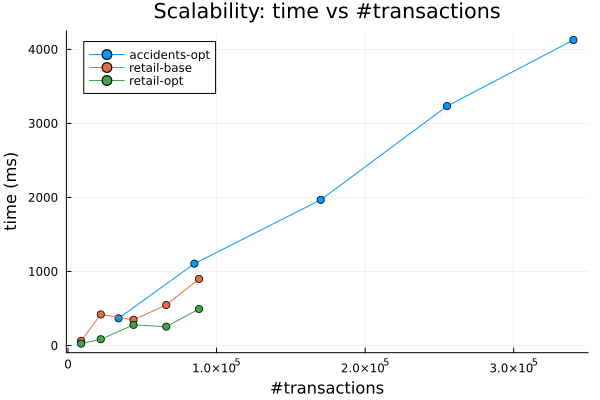
\includegraphics[width=0.88\linewidth]{../experiments/figures/scalability.png}
    \caption{Khả năng mở rộng theo số lượng giao dịch.}
    \label{fig:scalability}
\end{figure}

\subsection{Ảnh hưởng của độ dài giao dịch}

Thí nghiệm cuối dùng dữ liệu tổng hợp 20,000 giao dịch, 100 item, minsup $0.03$, và tăng độ dài giao dịch trung bình từ 5 đến 25. Bảng \ref{tab:txnlen} cho thấy thời gian tăng mạnh khi độ dài trung bình đạt 20 và 25.

\begin{table}[H]
    \centering
    \caption{Ảnh hưởng của độ dài giao dịch trung bình lên thời gian chạy FP-Max.}
    \label{tab:txnlen}
    \begin{tabular}{r r r}
        \toprule
        AvgLen & Time ms & \#Tối đại \\
        \midrule
        5 & 276.31 & 100 \\
        10 & 636.31 & 100 \\
        15 & 1349.64 & 100 \\
        20 & 19213.50 & 4,950 \\
        25 & 30039.70 & 4,950 \\
        \bottomrule
    \end{tabular}
\end{table}

\begin{figure}[H]
    \centering
    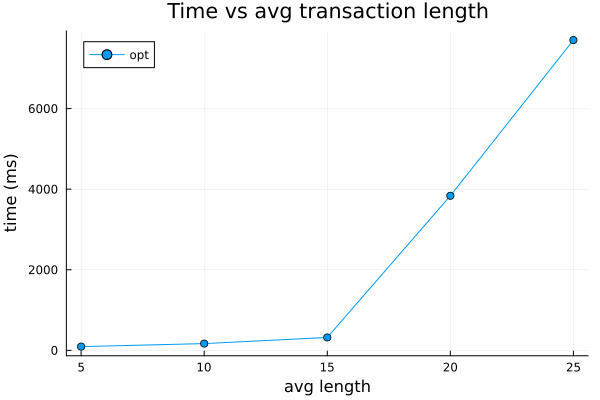
\includegraphics[width=0.82\linewidth]{../experiments/figures/txnlen.png}
    \caption{Thời gian chạy FP-Max khi tăng độ dài giao dịch trung bình.}
    \label{fig:txnlen}
\end{figure}

Kết quả này phù hợp với lý thuyết: giao dịch dài làm tăng xác suất các item cùng xuất hiện, làm FP-tree dày hơn và số tập tối đại tăng. Khi output size nhảy từ 100 lên 4,950 tối đại (giữa độ dài 15 và 20), thời gian cũng nhảy từ 1349.64 ms lên 19213.50 ms, tức tăng theo bậc lớn hơn nhiều so với mức tăng tuyến tính của độ dài giao dịch; Hình \ref{fig:txnlen} minh hoạ rõ bước nhảy này, đúng với cận mũ ở trường hợp xấu khi số tối đại $M$ bùng nổ.

\subsection{Nhận xét và hướng tối ưu tiếp theo}

Thực nghiệm cho thấy cài đặt FP-Max của nhóm đúng so với SPMF FPMax trên mọi cấu hình kiểm tra. Điểm mạnh quyết định là FP-Max trực tiếp hoàn tất trong những vùng mà baseline naive-maximal không khả thi --- toàn bộ Accidents và các ngưỡng thấp trên dữ liệu dày --- nhờ chỉ giữ biểu diễn tối đại và tỉa theo siêu tập. Trên dữ liệu dày như Chess và Mushrooms ở minsup thấp, FP-Max nhanh hơn baseline nhiều lần và cấp phát ít hơn rõ rệt.

Điểm yếu có hai mức. So với baseline, FP-Max chậm hơn trên dữ liệu thưa (Retail, T10I4D100K) vì phép tỉa ít tác dụng còn chi phí cài đặt cao. So với SPMF, FP-Max chậm hơn trên hầu hết cấu hình lớn. Nguyên nhân chính nằm ở cài đặt: FP-Max hiện dùng FP-tree với node \texttt{String} và tính lại support cho từng MFI bằng một lần quét toàn cơ sở dữ liệu.

Từ đó, hai hướng tối ưu cụ thể có thể làm tiếp. Thứ nhất, chuyển FP-Max sang dùng cấu trúc cây mã hoá số nguyên như \texttt{FPGrowthOpt} (header và children typed, \texttt{@inbounds}) để loại chi phí \texttt{String} trong hot loop. Thứ hai, mang support theo trong quá trình khai thác để bỏ hẳn bước tính lại support cho từng MFI ở cuối, vốn tốn một lần quét dữ liệu mỗi tối đại. Ngoài ra, có thể thay danh sách MFI tuyến tính bằng một MFI-tree để phép kiểm tra siêu tập có chi phí dưới tuyến tính, và song song hoá các nhánh conditional tree độc lập.

\section{Ứng dụng}

\subsection{Bài toán phân tích giỏ hàng}

Ứng dụng được chọn là phân tích giỏ hàng (Market Basket Analysis). Với mỗi giao dịch là một hoá đơn mua hàng, frequent itemsets cho biết các nhóm sản phẩm thường xuất hiện cùng nhau. Từ các itemset phổ biến, ta sinh luật kết hợp dạng $X \Rightarrow Y$, trong đó $X$ là vế trái, $Y$ là vế phải và $X \cap Y = \emptyset$.

Ba chỉ số được dùng để đánh giá luật là support, confidence và lift:
\[
    \operatorname{conf}(X \Rightarrow Y) =
    \frac{\operatorname{sup}(X \cup Y)}{\operatorname{sup}(X)}
\]
và
\[
    \operatorname{lift}(X \Rightarrow Y) =
    \frac{\operatorname{conf}(X \Rightarrow Y)}{\operatorname{sup}_{rel}(Y)}.
\]
Confidence đo xác suất mua $Y$ khi đã mua $X$. Lift đo mức tăng so với xác suất mua $Y$ độc lập. Nếu lift lớn hơn 1, $X$ và $Y$ có xu hướng xuất hiện cùng nhau nhiều hơn kỳ vọng ngẫu nhiên \cite{Agrawal1993AssociationRules}.

\subsection{Dữ liệu và thiết lập}

Nhóm sử dụng tập \texttt{data/groceries.txt}, gồm 9,835 giao dịch và 169 mặt hàng. Độ dài giao dịch trung bình là 4.41 item, giao dịch dài nhất có 32 item. Vì tên mặt hàng trong Groceries có thể chứa khoảng trắng, dữ liệu được tách theo dấu phẩy trước khi đưa vào thuật toán FP-Growth của nhóm. Thiết lập khai thác là:

\begin{itemize}
    \item minsup $= 0.01$, tương đương ít nhất $\lceil 0.01 \times 9835 \rceil = 99$ giao dịch.
    \item minconf $= 0.3$.
    \item Luật được sắp theo lift giảm dần; nếu lift bằng nhau thì ưu tiên confidence cao hơn.
\end{itemize}

Với thiết lập này, thuật toán tìm được 333 frequent itemsets và sinh 125 luật thoả minconf.

\subsection{Top-10 luật theo lift}

Bảng \ref{tab:grocery-rules} trình bày 10 luật có lift cao nhất. Support trong bảng là support tương đối.

\begin{table}[H]
    \centering
    \small
    \begin{tabular}{|p{5.0cm}|p{3.2cm}|r|r|r|}
        \hline
        Vế trái $X$ & Vế phải $Y$ & Support & Confidence & Lift \\
        \hline
        citrus fruit + other vegetables & root vegetables & 0.0104 & 0.3592 & 3.2950 \\
        \hline
        other vegetables + tropical fruit & root vegetables & 0.0123 & 0.3428 & 3.1448 \\
        \hline
        beef & root vegetables & 0.0174 & 0.3314 & 3.0404 \\
        \hline
        citrus fruit + root vegetables & other vegetables & 0.0104 & 0.5862 & 3.0296 \\
        \hline
        root vegetables + tropical fruit & other vegetables & 0.0123 & 0.5845 & 3.0210 \\
        \hline
        other vegetables + whole milk & root vegetables & 0.0232 & 0.3098 & 2.8421 \\
        \hline
        curd + whole milk & yogurt & 0.0101 & 0.3852 & 2.7614 \\
        \hline
        rolls/buns + root vegetables & other vegetables & 0.0122 & 0.5021 & 2.5949 \\
        \hline
        root vegetables + yogurt & other vegetables & 0.0129 & 0.5000 & 2.5841 \\
        \hline
        tropical fruit + whole milk & yogurt & 0.0151 & 0.3582 & 2.5675 \\
        \hline
    \end{tabular}
    \caption{Top-10 luật kết hợp trên Groceries theo lift, với minsup $=0.01$ và minconf $=0.3$.}
    \label{tab:grocery-rules}
\end{table}

\subsection{Diễn giải kinh doanh}

Các luật mạnh nhất tập trung quanh nhóm rau củ, sữa và sữa chua. Luật ``citrus fruit + other vegetables $\Rightarrow$ root vegetables'' có lift 3.2950, nghĩa là trong các giỏ hàng đã có trái cây họ cam chanh và rau khác, khả năng xuất hiện root vegetables cao hơn khoảng 3.3 lần so với tần suất nền của root vegetables. Đây là tín hiệu phù hợp cho gợi ý mua kèm hoặc bố trí kệ gần nhau giữa nhóm rau củ và trái cây tươi.

Luật ``beef $\Rightarrow$ root vegetables'' có confidence 0.3314 và lift 3.0404. Về mặt kinh doanh, người mua thịt bò có xu hướng mua thêm rau củ dùng cho món hầm, súp hoặc bữa ăn chính. Siêu thị có thể dùng luật này để thiết kế combo nguyên liệu hoặc coupon giảm giá chéo.

Nhóm luật liên quan tới \textit{whole milk}, \textit{curd} và \textit{yogurt} cho thấy các sản phẩm sữa có quan hệ đồng mua rõ. Ví dụ ``curd + whole milk $\Rightarrow$ yogurt'' có confidence 0.3852 và lift 2.7614. Luật này phù hợp cho gợi ý trong giỏ hàng trực tuyến: khi khách đã chọn curd và whole milk, hệ thống có thể đề xuất yogurt như một sản phẩm bổ sung.

Một điểm cần lưu ý là support của các luật top lift chỉ quanh 1--2.3\%. Các luật này có ý nghĩa định hướng gợi ý theo ngữ cảnh, nhưng không nên xem là luật bao phủ phần lớn khách hàng. Nếu mục tiêu là khuyến mãi diện rộng, cần cân bằng lift với support tuyệt đối và lợi nhuận của từng sản phẩm.


\section{Kết luận}
\label{sec:conclusion}

Đồ án đã hoàn thành việc nghiên cứu, cài đặt và đánh giá thuật toán FP-Max cho bài toán khai thác tập phổ biến tối đại. Về lý thuyết, báo cáo trình bày các định nghĩa cốt lõi của FIM, tính chất Apriori, cấu trúc FP-tree làm nền, và phần trọng tâm về FP-Max: danh sách MFI, phép tỉa theo siêu tập, shortcut single-path và phân tích độ phức tạp. Hai ví dụ tay minh hoạ FP-Max trên cả trường hợp cơ sở (cập nhật danh sách MFI) lẫn tình huống đặc biệt (phép tỉa bỏ qua nguyên một nhánh).

Về cài đặt, nhóm xây dựng package Julia \texttt{FrequentItemsetMining} gồm FP-Growth (bản cơ bản và bản tối ưu mã hoá số nguyên), một baseline naive-maximal khai thác toàn bộ tập phổ biến rồi lọc tối đại, và FP-Max khai thác trực tiếp có danh sách MFI và tỉa theo siêu tập. Output được giữ tương thích với định dạng SPMF để thuận tiện kiểm thử và đối chiếu.

Về thực nghiệm, kết quả correctness đạt \texttt{match\_ratio = 1.0} và \texttt{support\_mismatch = 0} so với SPMF FPMax trên mọi cấu hình benchmark được kiểm tra. Điểm mạnh quyết định của FP-Max trực tiếp là chạy được trong những vùng mà baseline naive-maximal không khả thi --- toàn bộ Accidents và các ngưỡng thấp trên dữ liệu dày --- nhờ chỉ giữ biểu diễn tối đại và tỉa không gian tìm kiếm. Trên dữ liệu dày, FP-Max còn nhanh hơn baseline nhiều lần, ví dụ khoảng 8.68 lần trên Chess tại minsup $0.8$ và 4.84 lần trên Mushrooms tại minsup $0.25$. Tuy vậy, trên dữ liệu thưa (Retail, T10I4D100K) FP-Max chậm hơn baseline vì phép tỉa ít tác dụng còn chi phí cài đặt cao, và nhìn chung vẫn chậm hơn SPMF.

Phần ứng dụng trên Groceries dùng bộ máy khai thác đầy đủ tập phổ biến (vì sinh luật cần support của mọi itemset) để tạo các luật kết hợp có ý nghĩa thực tế, chẳng hạn các luật liên quan tới \textit{root vegetables}, \textit{other vegetables}, \textit{whole milk} và \textit{yogurt}. Các luật này có thể hỗ trợ gợi ý sản phẩm, bố trí kệ hàng và thiết kế combo.

Các hạn chế còn lại của đồ án gồm: cài đặt FP-Max hiện dùng FP-tree với node \texttt{String} và tính lại support cho từng MFI bằng một lần quét toàn cơ sở dữ liệu, khiến nó chậm trên dữ liệu thưa; baseline naive-maximal phải skip nhiều cấu hình do nguy cơ bùng nổ. Trong tương lai, nhóm có thể chuyển FP-Max sang cấu trúc cây mã hoá số nguyên như bộ máy tối ưu, mang support theo trong quá trình khai thác để bỏ bước tính lại, thay danh sách MFI tuyến tính bằng một MFI-tree cho phép kiểm tra siêu tập dưới tuyến tính, và song song hoá các nhánh conditional tree độc lập.



% References
\input{ref/ref.tex}

% Appendix
% \appendix
% Add \cleardoublepage to move appendices to next page.
% \section{Phụ lục: Hướng dẫn tái lập}
\label{sec:appendix-repro}

Phụ lục này tóm tắt các bước tái lập toàn bộ mã nguồn, kiểm thử và thực nghiệm của đồ án. Nội dung tương ứng với tệp \texttt{README.md} trong kho mã nguồn; mọi lệnh đều chạy từ thư mục gốc của repo. Mã nguồn đầy đủ tại \href{https://github.com/p1neapplechoco/dma-lab2.git}{\texttt{github.com/p1neapplechoco/dma-lab2}}.

\subsection{Cấu trúc thư mục}

\begin{itemize}
    \item \texttt{src/}: package Julia \texttt{FrequentItemsetMining} (FP-Max và baseline naive-maximal, bộ máy nền FP-Growth cơ bản và tối ưu, sinh luật kết hợp, I/O).
    \item \texttt{main.jl}: giao diện dòng lệnh.
    \item \texttt{test/}: bộ kiểm thử correctness và benchmark.
    \item \texttt{experiments/}: harness thực nghiệm Chương \ref{sec:evaluation} và ứng dụng Chương \ref{sec:application}.
    \item \texttt{data/}: CSDL toy, benchmark và Groceries.
    \item \texttt{docs/Report.pdf}: báo cáo.
    \item \texttt{Project.toml}, \texttt{Manifest.toml}: khai báo và khoá phiên bản phụ thuộc.
\end{itemize}

Đồ án không sử dụng bất kỳ thư viện FIM có sẵn nào; SPMF chỉ được gọi như một công cụ hộp đen để đối chiếu kết quả ở Chương \ref{sec:evaluation}.

\subsection{Môi trường và cài đặt}

Yêu cầu Julia $\geq 1.9$ (đã kiểm thử trên Julia 1.12). Cách khuyến nghị là dùng \texttt{juliaup} — trình quản lý phiên bản chính thức của Julia:

\begin{lstlisting}[language=bash, caption={Cài Julia bằng juliaup (Linux/macOS) và ghim phiên bản.}]
curl -fsSL https://install.julialang.org | sh
juliaup add 1.12      # optional: pin the tested version
julia --version       # expected: julia version 1.12.x (or >= 1.9)
\end{lstlisting}

Trên Windows có thể cài từ Microsoft Store (tìm ``Julia'') hoặc chạy \texttt{winget install julia -s msstore}. Sau khi có Julia, cài phụ thuộc theo \texttt{Manifest.toml} đã khoá để đảm bảo tái lập:

\begin{lstlisting}[language=bash, caption={Cài đặt phụ thuộc.}]
julia --project=. -e 'using Pkg; Pkg.instantiate()'
\end{lstlisting}

\subsection{Chạy chương trình}

Giao diện dòng lệnh nhận đường dẫn dữ liệu, ngưỡng minsup tương đối, thuật toán và đường dẫn output (tùy chọn):

\begin{lstlisting}[language=bash, caption={Cú pháp dòng lệnh.}]
julia --project=. main.jl <input_path> <minsup> [fp-growth|fp-growth-opt|fp-max|rules] [output_path]
\end{lstlisting}

Ví dụ khai thác tập phổ biến tối đại bằng FP-Max trên CSDL toy với minsup $0.6$ (kết quả $\{1,3\}:3$, $\{2,3,5\}:3$):

\begin{lstlisting}[language=bash, caption={Khai thác tập tối đại bằng FP-Max.}]
julia --project=. main.jl data/toy/test_1.txt 0.6 fp-max output.txt
\end{lstlisting}

Đầu vào theo định dạng SPMF (mỗi giao dịch một dòng, item cách nhau bằng khoảng trắng; parser cũng chấp nhận dòng có dấu phẩy). Đầu ra theo dạng \texttt{item1 item2 ... \#SUP: support\_count}.

Chế độ \texttt{rules} sinh trực tiếp luật kết hợp (lift $> 1$, sắp theo lift giảm dần) từ tập phổ biến. Ngưỡng confidence đặt qua biến môi trường \texttt{MINCONF} (mặc định $0.2$), số luật in ra qua \texttt{TOPK} (mặc định $10$). Với dữ liệu mà tên item chứa khoảng trắng (ví dụ Groceries), đặt \texttt{SEP=comma} để parser chỉ tách theo dấu phẩy:

\begin{lstlisting}[language=bash, caption={Sinh luật kết hợp trên Groceries.}]
SEP=comma julia --project=. main.jl data/groceries.txt 0.01 rules rules.csv
\end{lstlisting}

Lệnh trên tái tạo đúng kết quả phần ứng dụng: $333$ frequent itemsets và $231$ luật có lift lớn hơn $1$.

\subsection{Kiểm thử}

\begin{lstlisting}[language=bash, caption={Chạy bộ kiểm thử tự động.}]
julia --project=. test/runtests.jl
\end{lstlisting}

Bộ kiểm thử gồm: kiểm tra parser ba định dạng; FP-Growth và FP-Max trên CSDL toy ở Chương \ref{sec:example}; đối chiếu bản tối ưu với bản cơ bản trên năm CSDL (hai toy và ba benchmark: chess, mushrooms, retail); kiểm tra sinh luật kết hợp; và benchmark đối chiếu base/opt trên chess. Các tỉ lệ tốc độ/bộ nhớ in trong dòng \texttt{[bench]} là số đo on-the-fly, phụ thuộc máy và lần chạy (JIT warm-up, GC) nên có thể dao động, không nhất thiết trùng với số liệu cố định trong báo cáo.

\subsection{Tái lập thực nghiệm Chương 4}

Thực nghiệm cần SPMF (làm chuẩn đối chiếu, yêu cầu Java $\geq 8$) và đầy đủ năm tập benchmark.

\begin{enumerate}
    \item Tải SPMF jar (bị \texttt{.gitignore} vì nặng):
\begin{lstlisting}[language=bash]
bash experiments/download_spmf.sh
\end{lstlisting}
    \item Tải dataset. Bốn tập chess, mushrooms, retail, T10I4D100K đã có sẵn trong \texttt{data/benchmark/}; bổ sung \texttt{accidents.txt} ($>25$ MB, không đưa vào repo) từ Google Drive vào \texttt{data/benchmark/}:

    \href{https://drive.google.com/drive/folders/1TuKapS5SYeWS1D8Zs4gegZHlqNAh36NE?usp=sharing}{Thư mục dữ liệu trên Google Drive}.
    \item Chạy thực nghiệm (sinh các file CSV trong \texttt{experiments/results/}):
\begin{lstlisting}[language=bash]
julia --project=. experiments/run_experiments.jl
\end{lstlisting}
    Có thể giới hạn tập dữ liệu qua biến môi trường, ví dụ bỏ qua accidents:
\begin{lstlisting}[language=bash]
EXP_DATASETS=chess,mushrooms,retail,T10I4D100K julia --project=. experiments/run_experiments.jl
\end{lstlisting}
    \item Đo peak RSS thật (sinh \texttt{experiments/results/memory.csv}):
\begin{lstlisting}[language=bash]
julia --project=. experiments/measure_memory.jl
\end{lstlisting}
    \item Sinh biểu đồ (vào \texttt{experiments/figures/}):
\begin{lstlisting}[language=bash]
julia --project=. experiments/make_figures.jl
\end{lstlisting}
\end{enumerate}

\subsection{Tái lập ứng dụng Chương 5}

Sinh luật kết hợp trên tập Groceries (minsup $0.01$, minconf $0.2$), in top-10 luật theo lift và ghi \texttt{experiments/results/rules\_groceries.csv}:

\begin{lstlisting}[language=bash, caption={Phân tích giỏ hàng.}]
julia --project=. experiments/application.jl
\end{lstlisting}

Kết quả mong đợi: $333$ frequent itemsets và $231$ luật có lift lớn hơn $1$. Kết quả này cũng đạt được trực tiếp qua chế độ \texttt{rules} của \texttt{main.jl} như ở mục Chạy chương trình.

\subsection{Tính tái lập}

Mọi dữ liệu tổng hợp dùng seed cố định (\texttt{experiments/datagen.jl}, seed $42$); \texttt{Manifest.toml} khoá toàn bộ phiên bản phụ thuộc. Số đếm (\#frequent itemsets, \#luật) và kết quả correctness là tất định nên chạy lại cho ra cùng giá trị; riêng các số đo thời gian và peak RSS có thể dao động theo máy và lần chạy do JIT, GC và tải hệ thống.

\end{document}